\documentclass[10pt]{article}
\usepackage[margin=1cm, bottom=2cm]{geometry}
\usepackage{tikz}
\usepackage[urlcolor=blue, colorlinks=true]{hyperref}
\usepackage{longtable}
\usepackage{multirow}
\usepackage{listings}
\usepackage{tabularx}
\usepackage{multicol}

\lstdefinestyle{lststyle}{numbers=left, escapechar=`}
\lstdefinelanguage{pseu}{keywords={if,for,while,and,procedure,Sudoku,repeat,times,
    Chromosome,Population,read,print,crossover,mutate,select,main,choose,segment_tree_choose,
    fitness,constructor,this,return}}

\begin{document}

\title{Report\\Assignment 2: Sudoku Solver}
\author{Timur Usmanov, B23-ISE-01}
\maketitle

\section{Introduction}
Find the complete source code and tests at \url{https://github.com/Error10556/IntroToAI2}.

\section{Algorithm overview}

This section provides insight into and comments on the EA solution. It considers
the overall flow of the algorithm and its specifics: the fitness function definition,
the variation operator implementations, the parameter values, and others.

From here, we will call a subgrid of $3\times3$ cells a \textit{block}.

\subsection{General algorthim flow}\label{flowlisting}

For this task, I decided to implement a Genetic Algorithm (GA), which is a kind of evolutionary algorithms.
The following pseudocode represents the actual execution steps of the program. For definitions and
concrete values of constants used in the code, refer to Table \ref{paramtable}.

\begin{lstlisting}[language=pseu, style=lststyle]
procedure main
    given := read the Sudoku from console
    population := create a Population from (given)
    while the population's best member is not the full solution
        crossover(population)
        mutate(population)
        select a fixed number of survivors(population)

        if the maximum fitness has not improved in the last MaxPatience iterations
            population := create a Population from (given)
            reset the counter of non-improving iterations
    print(population.best)

constructor of Population(given: Sudoku)
    this := empty Population
    repeat nMaxPopulation times
        initSudoku := fill each block in given correctly, but randomly
        this.add(Chromosome(initSudoku))

procedure crossover(population: Population)
    repeat nCrossovers times
        a := choose a Chromosome not chosen on this line so far
                randomly with weights = (fitness + `$\frac19$`(fitness_range))
        b := choose a Chromosome randomly uniformly
        repeat nChildren times
            child := a Chromosome whose Sudoku consists of 1-8 random blocks from a
                    and the other blocks from b
            population.add(child)
\end{lstlisting}
\pagebreak
\begin{lstlisting}[language=pseu, style=lststyle, firstnumber=last]
procedure mutate(population: Population)
    repeat nMutants times and then until the population size reaches nMaxPopulation
        mutant := choose and copy a Chromosome among the initial ones
                randomly with weights = (fitness)
        nMutations := choose a number in [1, nMaxMutations] randomly uniformly
        repeat nMutations times
            exchange any two non-initial digits in the same block
        population.add(mutant)
    
procedure select(population: Population)
    mxFit := fitness(population.best)
    while population.size > nMaxPopulation and population.size > nElites:
        victim := choose a Chromosome that is not in the top-(nElites) randomly
                with weights = (mxFit - fitness + `$\frac13$`fitness_range)
        population.remove(victim)
    while population.size > nMaxPopulation
        population.remove(population.worst)
\end{lstlisting}

Basically, the program initializes the population by randomly filling blocks
with permutations of numbers $1$ -- $9$ and repeatedly crosses over, mutates,
and reduces the population until the solution is found or there have been no
improvements for some time, in which case the program restarts.

\subsection{Weighted random choice optimization}
To efficiently (i.e. in $O(\log n)$ time) choose several \textit{distinct} elements from a set at random while also
giving more probability to certain items, I used a segment tree that supports
updates on a single node, summing on segments of the tree, and binary descent.

The choice procedure is as follows:

\begin{lstlisting}[language=pseu, style=lststyle]
procedure segment_tree_choose
    sz := the sum of all weights
    if sz = 0
        return -1
    rnd := randomly uniformly choose from [0, sz)
    pos := the root node
    while pos represents a segment, not an individual element
        if rnd < the sum in the left half of segment at pos
            pos := left half of segment at pos
        else
            rnd := rnd - the sum in the left half of segment at pos
            pos := right half of segment at pos
    return the index of element at pos
\end{lstlisting}

\subsection{Chromosome representation}\label{repr}

We define a \textit{zone} as a row, a column, or a block.

\textbf{\texttt{Chromosome}} instances consist of:

\begin{itemize}
    \item a $9\times9$ grid of digits from $0$ to $9$, where $0$ represents an
        empty cell;
    \item a $9\times9$ grid of boolean flags that mark immutable cells (the cells
        that are filled initially);
    \item the counter of non-empty cells;
    \item the \textit{linear counter} of mistakes;
    \item the \textit{quadratic counter} of mistakes;
    \item 27 \textbf{\texttt{Digit Counter}}s: one for each of the 9 rows, columns, and blocks;
    \item the hash-sum for fast comparison.
\end{itemize}

In a single zone, a \textit{linear counter} of mistakes holds the minimum number of cells that have to be
emptied for the zone to contain no contradictions. A \textit{quadratic counter} of mistakes for a single zone
holds the number of distinct pairs of cells that contain the same digit. These are maintained by \textbf{\texttt{Digit Counter}}s.

The \textit{linear counter} of mistakes holds the sum of linear counters across all \textit{zones}. Similarly,
the \textit{quadratic counter} is the sum of all quadratic counters in all zones. In the present implementation,
the quadratic counter is not used, but it was on previous versions.

A \textbf{\texttt{Digit Counter}} maintains the quantity of every digit in a zone and
the zone's linear and quadratic counters.

The hash-sum is a polynomial hash of length 81 with coefficient 10; it is updated
efficiently (in $O(1)$) after each modification. The powers of 10 needed for
fast updates are calculated at compile-time to further reduce the runtime overhead.

\subsection{Fitness function}\label{fitness}

In the above solution, the \textit{fitness} function of a chromosome equals
\[81 - (\textrm{The value of the linear counter of mistakes}).\]
This formula does not punish the chromosome too harshly for disadvantageous mutations,
allowing for more genetic diversity and flexibility; for example, it is possible for a
long series of mutations to occur (without the chromosome being discarded) that would lead
to a nontrivial improvement. This formula gives more chances to avoid local maximums.

Thus, the maximum fitness is obviously $81$ and is only possible if the solution
is absolutely correct. The minimum fitness is achieved when the sudoku field is
filled with one digit. Then, in each zone the linear counter of mistakes holds the value 8
(the maximum possible value, obviously; see the definition in Sec. \ref{repr}),
and the total punishment is $27\cdot8=216$ since there are 27 zones. That gives
the minimum value of the fitness function $81-27\cdot8=-135$.

The \texttt{fitness\_range} value used in the pseudocode (Sec. \ref{flowlisting}) is,
therefore, $81-(-135)=216$.

Previously, another formula was used:
\[(\textrm{No. of non-empty cells}) - (\textrm{The quadratic counter of mistakes})
    - (\textrm{5 points if the sudoku contains a contradiction, else 0}).\]
It provided fast improvements of chromosomes at the start of the evolution.
However, this function made it unlikely for significantly long chains of mutations to
occur, limiting the exploration of the solution space. So the evolution usually
``got stuck'' at $79/81$ maximum fitness and never reached a complete solution.

\subsection{Variation operators}
Here we will discuss the reasons behind design choices made in the operators.
For a brief overview, see the pseudocode listing in Sec. \ref{flowlisting}.

\subsubsection{General ideas}
The general philosophy in this algorithm is to somehow guarantee that at least
the blocks will always be contradiction-free. The following considerations all
aim at maintaining the correctness of blocks.

Another key idea is to use a data structure such as an \texttt{ordered\_set} in \texttt{C++}
to store the chromosomes in a population. First, this approach allows for easy
access to the best and the worst chromosomes of the population if we primarily
order them by fitness. Second, this data structure automatically discards duplicate
chromosomes, which promotes genetic diversity that is necessary to search for
the correct solution in a wider range.

\subsubsection{Mutation}
No mutation should be able to create a contradiction within a block, i.e.
exchange different digits across different blocks or reassign a singular digit.
Therefore, we only allow swaps within one block.

We pick the base chromosomes for mutations randomly, but with slightly more preference
to fit individuals. This heuristic allows to quickly advance the overall fitness
of the population, especially at early stages. In fact, this design choice may
contradict our motivation for using a lenient fitness function (see Sec. \ref{fitness})
at the final iterations, which could cause convergence to local maxima. However,
the advantage of performance boost at early iterations outweighs this drawback.

\subsubsection{Crossover}
Again, no crossover should be able to create a contradiction within a block. Therefore,
we only cross chromosomes over via borrowing whole blocks from the parents.

When choosing parents, we pick one using weighted randomness and the other using
simple, uniform randomness. That is because, on the one hand, we want the child
to be fit, i.e. containing as few mistakes in its rows and columns as possible.
If one parent contains few errors, then the blocks taken from that parent will also
be less likely to form contradictions.
On the other hand, we want to explore as much of the solution space as possible.
So the second parent is chosen at random to try to find a new, unexplored combination
that would lead the evolution to the absolute solution.

When choosing the first parent (the one chosen with weighted randomness), we do
not want to completely exclude the chromosomes with low fitness. Therefore, the
weights assigned to the chromosomes are increased by $\frac19$ of the fitness range ($\frac19\cdot216=24$).

\subsubsection{Selection}
We generally want to discard the unfit chromosomes, that is why we assign more
weight and are likely to remove those which differ from the current maximum more.
To increase randomness and diversity among chromosomes, we add $\frac13$ of the
fitness range ($\frac13\cdot216=72$) to the weights.

However, we have to preserve some amount of the most fit chromosomes, so we always
leave \texttt{nElites} ones at the top, unless no more ``non-elite'' chromosomes
are left to discard.

\subsection{Parameters}

\begin{table}[!h]
    \begin{center}
        \begin{tabularx}{0.9\textwidth}{|>{\centering\arraybackslash}X|c|c|c|}
        \hline
        \textbf{Parameter definition} & \textbf{Name} & \textbf{Code name} & \textbf{Value} \\\hline
        The maximum number of iterations that do not improve the best fitness & \texttt{MaxPatience} & \texttt{MaxPatience} & 1000 \\\hline
        The maximum and preferred number of chromosomes in the population & \texttt{nMaxPopulation} & \texttt{MaxPopulation} & 500 \\\hline
        The number of times a pair of chromosomes is chosen for a crossover & \texttt{nCrossovers} & \texttt{noLuckyChromosomes} & 166 \\\hline
        The minimum number of mutants entering the population each iteration & \texttt{nMutants} & \texttt{minMutationCount} & 500 \\\hline
        The upper bound for the number of mutations per mutant & \texttt{nMutations} & \texttt{mutationMax} & 5 \\\hline
        The number of best chromosomes never discarded & \texttt{nElites} & \texttt{elites} & 100 \\\hline
    \end{tabularx}
    \end{center}
    \caption{Constant parameters used by the algorithm}\label{paramtable}
\end{table}

Table \ref{paramtable} contains the definitions, names (in the report and in the code),
and the values of parameters that regulate the intensity of some operations. The
values have been determined to be near-optimal empirically.

\section{Statistics}
This section lists the maximum and the average chromosome fitnesses at the
last iterations of the genetic algorithm.

\subsection{Test cases}
The solution has been tested on 180 tests: 10 tests per each difficulty level, of
which there were 18. The \textit{difficulty level} of a test case is considered
to be the number of initially given digits. The lowest number of given digits
I could find is 23, so the levels' range is $[23..40]$.

The test cases can be found at \url{https://github.com/Error10556/IntroToAI2/tree/main/tests10}.
The files follow a naming convention \texttt{testXX-YY}, where \texttt{XX} is the number
of initially given digits and \texttt{YY} is the test case index within that difficulty.

\subsection{Results}

Obviously, in the present case, the maximum fitness at the last iteration is going to be 81, which
is confirmed by every program execution.

\begin{table}[t]
    \begin{center}
        \begin{tabular}{|c|c|c|c|c|c|c|c|c|c|c|c|}
            \hline
            \multirow{2}{2.25cm}{Difficulty level} & \multicolumn{10}{c|}{Test case} & \multirow{2}{1.3cm}{Mean} \\\cline{2-11}
            & 1 & 2 & 3 & 4 & 5 & 6 & 7 & 8 & 9 & 10 &\\\hline
            23 & 68.824 & 67.746 & 67.198 & 68.534 & 67.99 & 67.702 & 67.252 & 67.31 & 67.598 & 67.806 & 67.796\\\hline
            24 & 68.16 & 68.22 & 67.076 & 67.732 & 66.544 & 67.564 & 66.904 & 68.342 & 66.426 & 69.254 & 67.6222\\\hline
            25 & 67.29 & 67.3 & 67.744 & 67.874 & 66.886 & 68.54 & 67.238 & 67.698 & 67.166 & 67.302 & 67.5038\\\hline
            26 & 68.58 & 66.708 & 67.588 & 68.042 & 67.576 & 68.122 & 66.952 & 67.446 & 67.98 & 67.512 & 67.6506\\\hline
            27 & 67.572 & 67.438 & 68.722 & 67.656 & 67.404 & 67.736 & 68.618 & 67.256 & 67.64 & 67.59 & 67.7632\\\hline
            28 & 67.888 & 67.93 & 67.168 & 67.168 & 67.142 & 67.776 & 68.244 & 67.204 & 67.054 & 67.204 & 67.4778\\\hline
            29 & 66.054 & 65.842 & 67.896 & 67.822 & 67.928 & 67.056 & 67.43 & 68.47 & 68.102 & 67.802 & 67.4402\\\hline
            30 & 66.606 & 67.77 & 68.188 & 68.796 & 68.252 & 69.356 & 67.886 & 68.174 & 68.178 & 66.91 & 68.0116\\\hline
            31 & 67.67 & 67.684 & 67.054 & 68.424 & 68.052 & 69.312 & 68.312 & 68.504 & 68.092 & 68.106 & 68.121\\\hline
            32 & 68.26 & 67.514 & 67.39 & 67.434 & 68.554 & 69.266 & 68.124 & 67.96 & 66.134 & 67.29 & 67.7926\\\hline
            33 & 67.258 & 68.478 & 67.562 & 68.162 & 68.938 & 67.532 & 68.374 & 68.186 & 68.008 & 67.894 & 68.0392\\\hline
            34 & 68.814 & 67.814 & 67.058 & 68.176 & 67.972 & 68.834 & 66.898 & 68.642 & 67.954 & 68.414 & 68.0576\\\hline
            35 & 67.552 & 68.55 & 68.092 & 68.142 & 67.318 & 67.878 & 67.888 & 67.084 & 68.254 & 68.97 & 67.9728\\\hline
            36 & 68.272 & 68.042 & 68.936 & 68.742 & 68.404 & 68.55 & 68.654 & 67.65 & 68.654 & 68.63 & 68.4534\\\hline
            37 & 68.488 & 67.96 & 67.324 & 67.944 & 67.328 & 66.52 & 68.25 & 68.458 & 67.802 & 67.434 & 67.7508\\\hline
            38 & 68.118 & 67.106 & 67.584 & 68.172 & 66.894 & 68.12 & 68.172 & 68.828 & 67.594 & 67.988 & 67.8576\\\hline
            39 & 68.07 & 67.88 & 68.114 & 67.594 & 67.102 & 67.03 & 68.094 & 67.922 & 68.34 & 68.168 & 67.8314\\\hline
            40 & 68.254 & 68.55 & 68.048 & 68.354 & 68.492 & 68.836 & 65.944 & 68.32 & 68.08 & 66.908 & 67.9786\\\hline
        \end{tabular}
    \end{center}
    \caption{The average chromosome fitnesses and the mean average for each difficulty}\label{tableavg}
\end{table}

The averages of fitnesses on last iterations can be found in Table \ref{tableavg}.

\begin{figure}[t]
    \begin{center}
        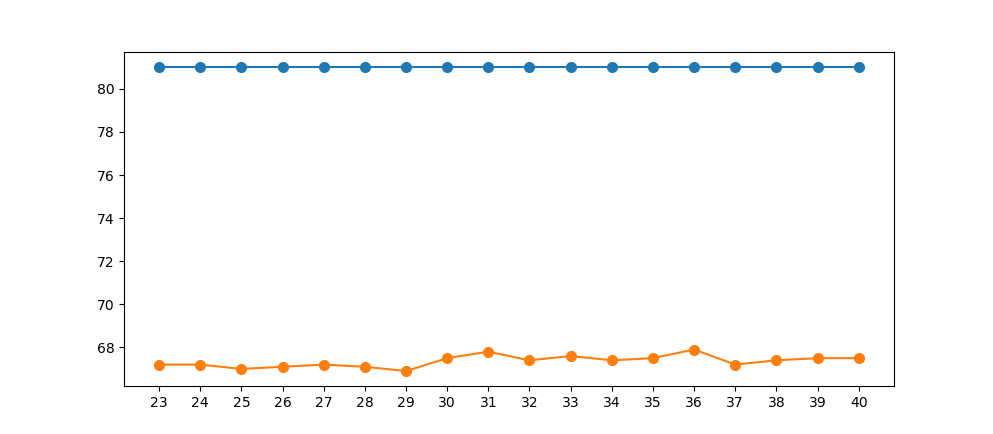
\includegraphics[scale=0.6]{Figure_Plot.png}
    \end{center}
    \caption{The plot of averages of average fitnesses and maximum fitnesses at every difficulty}\label{figPlot}
\end{figure}

\subsection{Discussion}
As is clear from Fig. \ref{figPlot}, the average fitness at the last iteration
does not depend on the difficulty of tests. Rather, it is always around 67 or 68, while
the most fit chromosome has a fitness value of 81.

\end{document}
